
\documentclass[11pt]{article}
\usepackage[utf8]{inputenc}
\usepackage{graphicx}
\usepackage{amsmath, amssymb}
\usepackage{geometry}
\usepackage{hyperref}
\usepackage{enumitem}
\usepackage{fancyhdr}
\usepackage{caption}
\pagestyle{fancy}
\fancyhf{}
\fancyhead[L]{GEANT4 Calorimeter Tutorial}
\fancyhead[R]{Dr. Ajay Kumar}
\fancyfoot[C]{\thepage}
\geometry{margin=1in}

\begin{document}

\begin{titlepage}
  \centering
  \vspace*{2cm}

  {\LARGE \bfseries GEANT4 Calorimeter Simulation and Analysis Tutorial \par}
  \vspace{1.5cm}

  {\Large Dr. Ajay Kumar\par}
  \vspace{0.5cm}
  Department of Physics\\
  Institute of Science, Banaras Hindu University\\
  \texttt{ajaykumar@bhu.ac.in}

  \vfill

  {\large \today\par}
\end{titlepage}

\section{Physics Motivation}

Calorimeters are essential tools in high-energy particle physics detectors. They are designed to absorb incoming particles and measure their energy via the resulting particle showers. This tutorial simulates the behavior of electromagnetic (EM) showers in a sampling calorimeter using the GEANT4 toolkit \cite{geant4_manual}.

Electromagnetic showers are cascades of particles—electrons, positrons, and photons—produced primarily through bremsstrahlung and pair production. The critical parameters that determine shower development are the initial particle energy, material properties like radiation length \( X_0 \), and the critical energy \( E_c \) below which ionization dominates over radiative processes \cite{pdg_calorimetry}.

In a sampling calorimeter:
\begin{itemize}
  \item \textbf{Absorber layers} (e.g., lead) induce shower multiplication.
  \item \textbf{Active layers} (e.g., scintillators) sample the energy deposit.
  \item The shower develops over multiple radiation lengths, with a longitudinal and radial spread.
\end{itemize}

The average longitudinal shower profile follows a Gamma distribution:
\begin{equation}
\frac{dE}{dt} = E_0 b \cdot \frac{(bt)^{a-1}e^{-bt}}{\Gamma(a)}
\end{equation}
where:
\begin{itemize}
    \item \( t = x / X_0 \) is the depth in radiation lengths,
    \item \( a \approx \ln(E_0 / E_c) \),
    \item \( b \approx 0.5 \),
    \item \( E_c \): material-dependent critical energy.
\end{itemize}

This model is well-established in detector design for experiments such as CMS, ATLAS, and upcoming facilities like the Electron-Ion Collider (EIC) \cite{cms_ecal_tdr, atlas_lar_tdr}.

\section{Simulation Overview}

GEANT4 is a C++-based toolkit developed at CERN for simulating the passage of particles through matter. Its modular structure allows accurate modeling of detector components and physics processes \cite{geant4_manual}.

\subsection*{GEANT4 Components}
\begin{itemize}
  \item \texttt{DetectorConstruction.cc}: Defines geometry and materials of absorber and scintillator layers.
  \item \texttt{PrimaryGeneratorAction.cc}: Configures the primary electron beam (energy, direction).
  \item \texttt{RunAction.cc}, \texttt{EventAction.cc}: Manage run-wise and event-wise actions (initialization, finalization).
  \item \texttt{SteppingAction.cc}: Intercepts simulation steps, records hits, energy deposits, and positions.
\end{itemize}

\subsection*{Geometry}
The calorimeter consists of multiple alternating layers:
\begin{itemize}
  \item \textbf{Absorber (Pb)}: Simulates electromagnetic interactions (e.g., bremsstrahlung).
  \item \textbf{Active (Scintillator)}: Detects energy through ionization.
  \item \textbf{Granularity}: Each layer is divided into small cells (\( \Delta x = \Delta y \sim 1\,\mathrm{cm} \)).
\end{itemize}

The detector dimensions and number of layers are tuned to fully contain showers up to ~100 GeV.

\section{ROOT Output and Data Products}

The simulation outputs a ROOT file containing histograms and trees that encode physical observables:

\subsection*{Histograms}
\begin{itemize}
  \item \textbf{hTotal (TH1D)}: Histogram of total deposited energy.
  \item \textbf{hLong (TH1D)}: Energy vs. layer index (longitudinal profile).
  \item \textbf{hRadial (TH1D)}: Energy vs. radial distance from shower axis.
  \item \textbf{hXY (TH2D)}: 2D heatmap of energy in the transverse XY plane.
  \item \textbf{TTree Hits}: Records position, layer ID, and deposited energy for each hit.
\end{itemize}

These observables are vital for understanding calorimeter resolution and response function.

\section{Python Analysis with \texttt{plot\_profiles.py}}

The ROOT data is analyzed using Python libraries such as \texttt{uproot}, \texttt{awkward}, and \texttt{matplotlib}. These allow histogram manipulation and fast plotting without needing a ROOT installation.

\subsection*{Generated Plots}
\vspace{-0.5em}
\begin{figure}[h!]
  \centering
  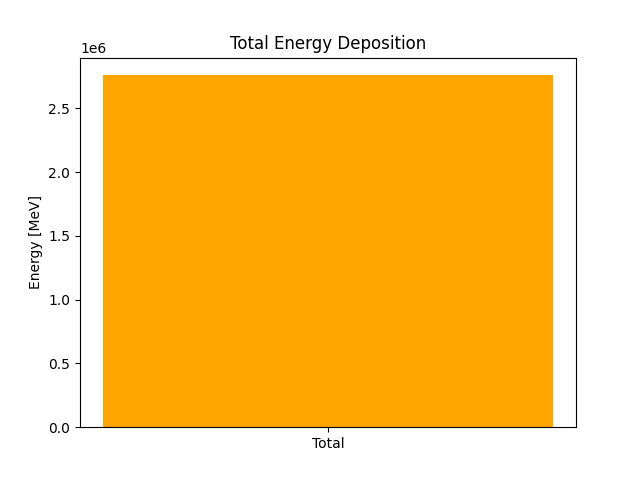
\includegraphics[width=0.6\textwidth]{figures/plot_total.png}
  \caption{Total energy deposited in the calorimeter}
\end{figure}

\begin{figure}[h!]
  \centering
  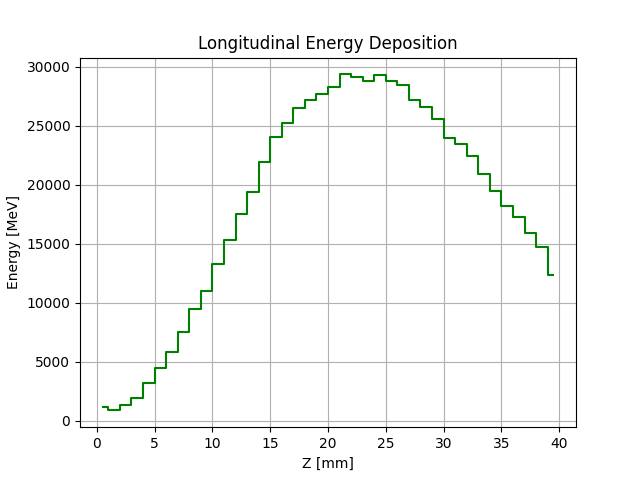
\includegraphics[width=0.6\textwidth]{figures/plot_longitudinal.png}
  \caption{Longitudinal energy deposition per layer}
\end{figure}

\begin{figure}[h!]
  \centering
  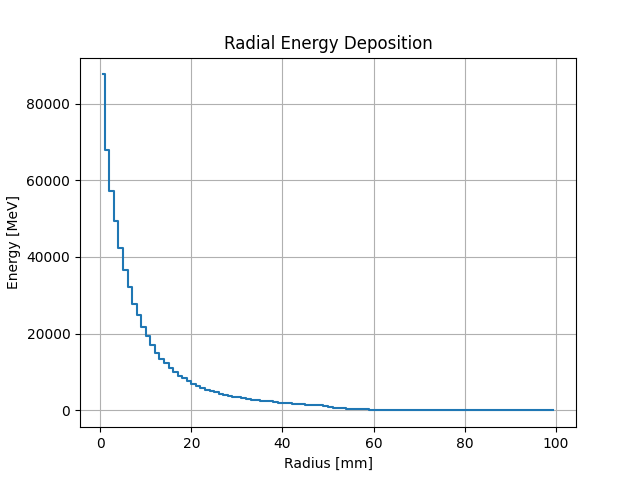
\includegraphics[width=0.6\textwidth]{figures/plot_radial.png}
  \caption{Radial distribution of deposited energy}
\end{figure}

\begin{figure}[h!]
  \centering
  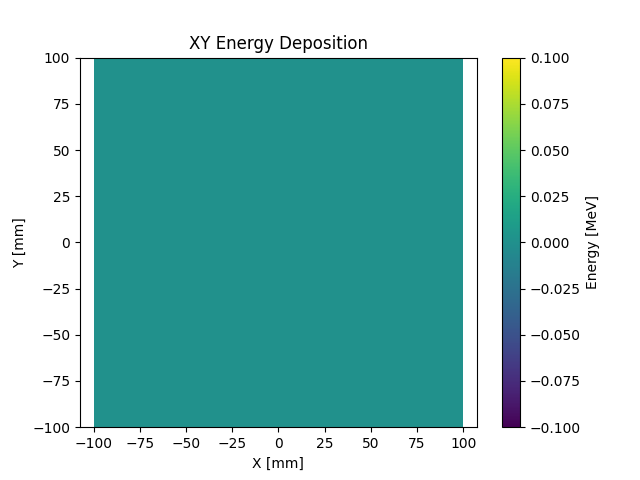
\includegraphics[width=0.6\textwidth]{figures/plot_xy.png}
  \caption{XY energy map at calorimeter front face}
\end{figure}

\subsection*{Sample Code}
\begin{verbatim}
import uproot
import matplotlib.pyplot as plt
file = uproot.open("build/output.root")
h = file["hTotal"].to_hist()
plt.bar(h.axes[0].centers, h.values())
plt.xlabel("Energy [MeV]")
plt.ylabel("Events")
plt.title("Total Deposited Energy")
plt.show()
\end{verbatim}

\section{Extending the Simulation}

This GEANT4 setup can be extended to:
\begin{itemize}
  \item Visualize XY energy maps at each depth slice.
  \item Export all hits to ntuples for ML analysis.
  \item Automate energy scans via scripts or Docker entrypoints.
\end{itemize}

\subsection*{Example Batch Run}
\begin{verbatim}
for E in 5 10 50 100; do
  ./CalorimeterSim -E $E -o output_$E.root
  python3 plot_profiles.py output_$E.root
done
\end{verbatim}

\section{Running with Docker (macOS/Linux)}

To ensure reproducibility and portability, we use a pre-built Docker image.

\subsection*{Step 1: Pull the Docker Image}
\begin{verbatim}
docker pull ajaykumar49/calorimeter-dev:snapshot3
\end{verbatim}

\subsection*{Step 2: Launch Container}
\begin{verbatim}
docker run -it -v $PWD:/work -w /work ajaykumar49/calorimeter-dev:snapshot3 /bin/bash
\end{verbatim}

\subsection*{Step 3: Run Simulation and Plot}
\begin{verbatim}
source /opt/geant4/bin/geant4.sh
cmake -B build -S . && make -C build
./build/CalorimeterSim
python3 plot_profiles.py build/output.root
\end{verbatim}

\section{Conclusion and Applications}

This exercise illustrates:
\begin{itemize}
  \item Physics of EM showers in sampling calorimeters
  \item Practical GEANT4 simulation and ROOT output
  \item Python-based post-processing and visualization
\end{itemize}

\textbf{Applications} include:
\begin{itemize}
  \item Optimizing detector design in collider experiments
  \item Modeling calorimeter response for ML training
  \item Jet substructure and tagging in heavy-ion physics
\end{itemize}

\section{References}
\begin{itemize}
  \item \label{geant4_manual}GEANT4 Collaboration, "GEANT4—A simulation toolkit", Nucl. Instrum. Meth. A 506 (2003) 250.
  \item \label{pdg_calorimetry}Particle Data Group, "Passage of particles through matter", \url{https://pdg.lbl.gov/2023/reviews/rpp2023-rev-passage-particles-matter.pdf}
  \item \label{cms_ecal_tdr}CMS Collaboration, ECAL Technical Design Report, CERN-LHCC-97-033.
  \item \label{atlas_lar_tdr}ATLAS Collaboration, Liquid Argon Calorimeter TDR, CERN-LHCC-96-041.
  \item \label{root_docs}ROOT User Guide, \url{https://root.cern/manual}
\end{itemize}

\end{document}
